\begin{frame}{Time, space and organization representation in multi-agent simulation}
\begin{columns}
\visible<1->{\begin{column}{.50\linewidth}
\vspace{.6cm}
\begin{figure}
    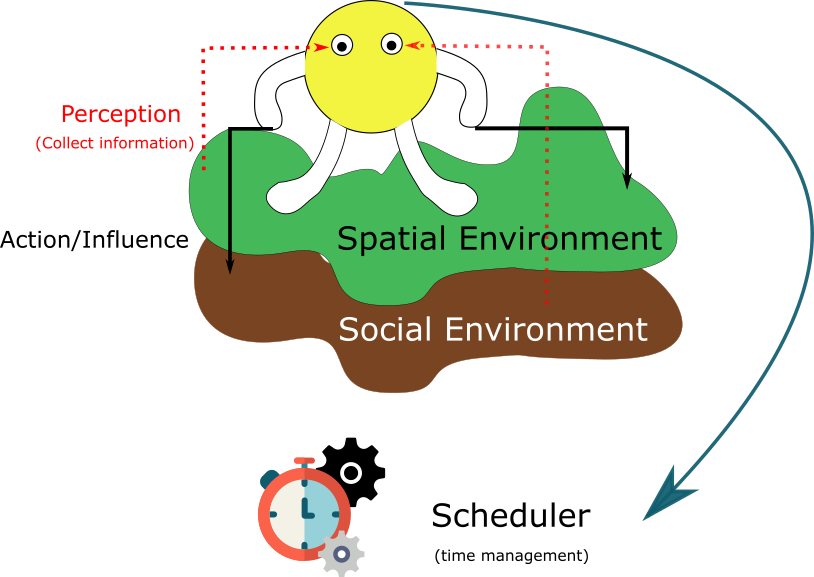
\includegraphics[width=.85\linewidth]{figures/before.png}
    \caption{MAS classical approach}
\end{figure}
\end{column}}
\visible<2->{
\begin{column}{.50\linewidth}
\begin{figure}
    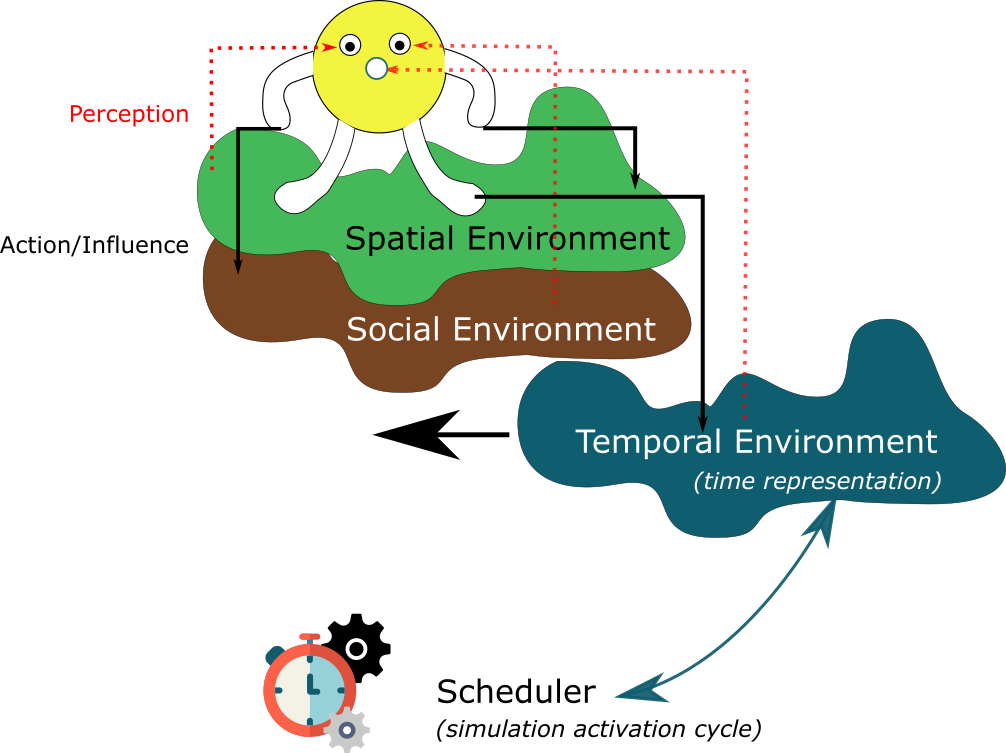
\includegraphics[width=\linewidth]{figures/after.png}
     \caption{Our proposition}
\end{figure}
\end{column}}
\end{columns}
\note{
\par Dans beaucoup d'approches dans les simulations multi-agents, l'espace comme les organisations sont modélisé sous la forme d'environnements. Ces environnements spatiales et sociales permettent aux agents de partager et d'accéder à des informations sur leur contexte d'activation spatial et social.
\par Contrairement à cela, de manière générale, le temps est abordé uniquement sous l'angle technique, en tant que mécanique de la simulation. Il est géré au niveau d'une entité de la plateforme de simulation appelé ordonnanceur. Le fonctionnement de l'ordonnanceur consiste à gérer le cycle d'activation de la simulation, en faisant s'écouler virtuellement le temps. L'ensemble des connaissances concernant le comportement temporel des agents est alors accessible et exploité uniquement par l'ordonnanceur de la simulation. 
\par Afin de permettre aux agents d'avoir une visibilité sur cette dynamique d'activation temporelle et de l'exploiter, nous proposons de compléter le fonctionnement de l'ordonnanceur de la simulation par un milieu d'interaction que nous appelons l'environnement temporel. Désormais, la gestion du temps au niveau de la simulation multi-agents se faire sur deux niveaux:
\begin{itemize}
    \item Au niveau de l'environnement temporel : qui sert de support permettant aux agents de partager et de percevoir les informations sur leur comportement temporel
    \item Au niveau de l'ordonnanceur de la simulation : qui gère l'écoulement du temps et le cycle d'activation de la simulation
\end{itemize}
}
    
\end{frame}

\begin{frame}{The Temporal Environment}{General architecture}
\par \textbf{Objective}: evolve multi-agent simulations in such a way as to consider time as a medium of interaction, in the same way as space or organisations.
\vspace{1cm}
\par \textbf{Proposition}:

\begin{columns}
\begin{column}{.3\linewidth}
\begin{figure}
    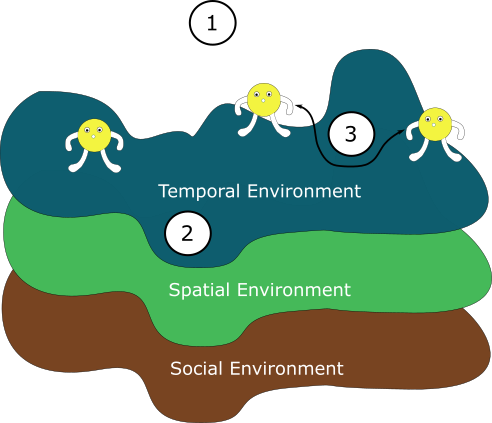
\includegraphics[width=\linewidth]{figures/temporalRepresentation.png}
\end{figure}
\end{column}
\begin{column}{.7\linewidth}
\begin{enumerate}
    \item The \textbf{Agent-Group-Role-Environment-Time (AGRET)} model
    \item The \textbf{temporal environment}\footnote{RALITERA, Tahina, PAYET, Denis, et COURDIER, Rémy. Toward a Temporal Environment for Multi-Agent Simulation. Journal of Communications, 2019, vol. 14, no 7.}
    \item The Influence-Reaction Model For Simulation (IRM4S) \footnote{MICHEL, Fabien. The IRM4S model: the influence/reaction principle for multiagent based simulation. In : Proceedings of the 6th international joint conference on Autonomous agents and multiagent systems. 2007. p. 1-3.}
\end{enumerate}
\end{column}
\end{columns}
\note{
Notre objectif est de faire évoluer les simulations multi-agents de manière à considérer le temps comme un milieu d'interaction, au même titre que l'espace ou les organisations. Ce nouveau milieu d'interaction s'appelle l'environnement temporel et peut se définir de manière très simple comme un espace dont la métrique est le temps. L'agent est capable de percevoir et d'agir sur son environnement temporel selon le modèle IRM4S, un modèle d'interaction de type influence/réaction spécialement conçu pour la simulation.
\par Pour mettre en place ce nouvel environnement au sein du système existant, nous proposons une méthodologie de conception permettant d’articuler les 3 dimensions spatiale, organisationnelle et temporelle. Nous appelons cette approche AGRET. AGRET étend l'approche AGRE en y rajoutant la prise en compte de l'environnement temporelle au même titre que les environnements spatiales et sociales. AGRE est elle même une extension du modèle générique d'organisation AGR qui rajoute la prise en compte de l'environnement spatiale à la prise en compte de la dimensions sociale qui est faite au niveau d'AGR.
}  
\end{frame}

\begin{frame}{The temporal Environment}{Structure}
\begin{columns}
\visible<1->{
\begin{column}{.33\linewidth}
\begin{figure}
    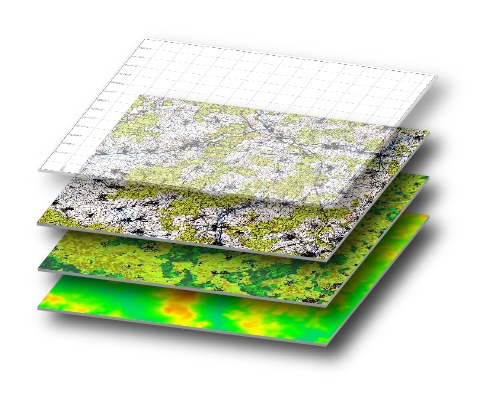
\includegraphics[width=\linewidth]{figures/space.png}
    \caption{The \textbf{spatial} environment structure.\medbreak \textit{Ex: GIS, grid, continuous space, etc.}}
\end{figure}
\end{column}
\begin{column}{.33\linewidth}
\begin{figure}
    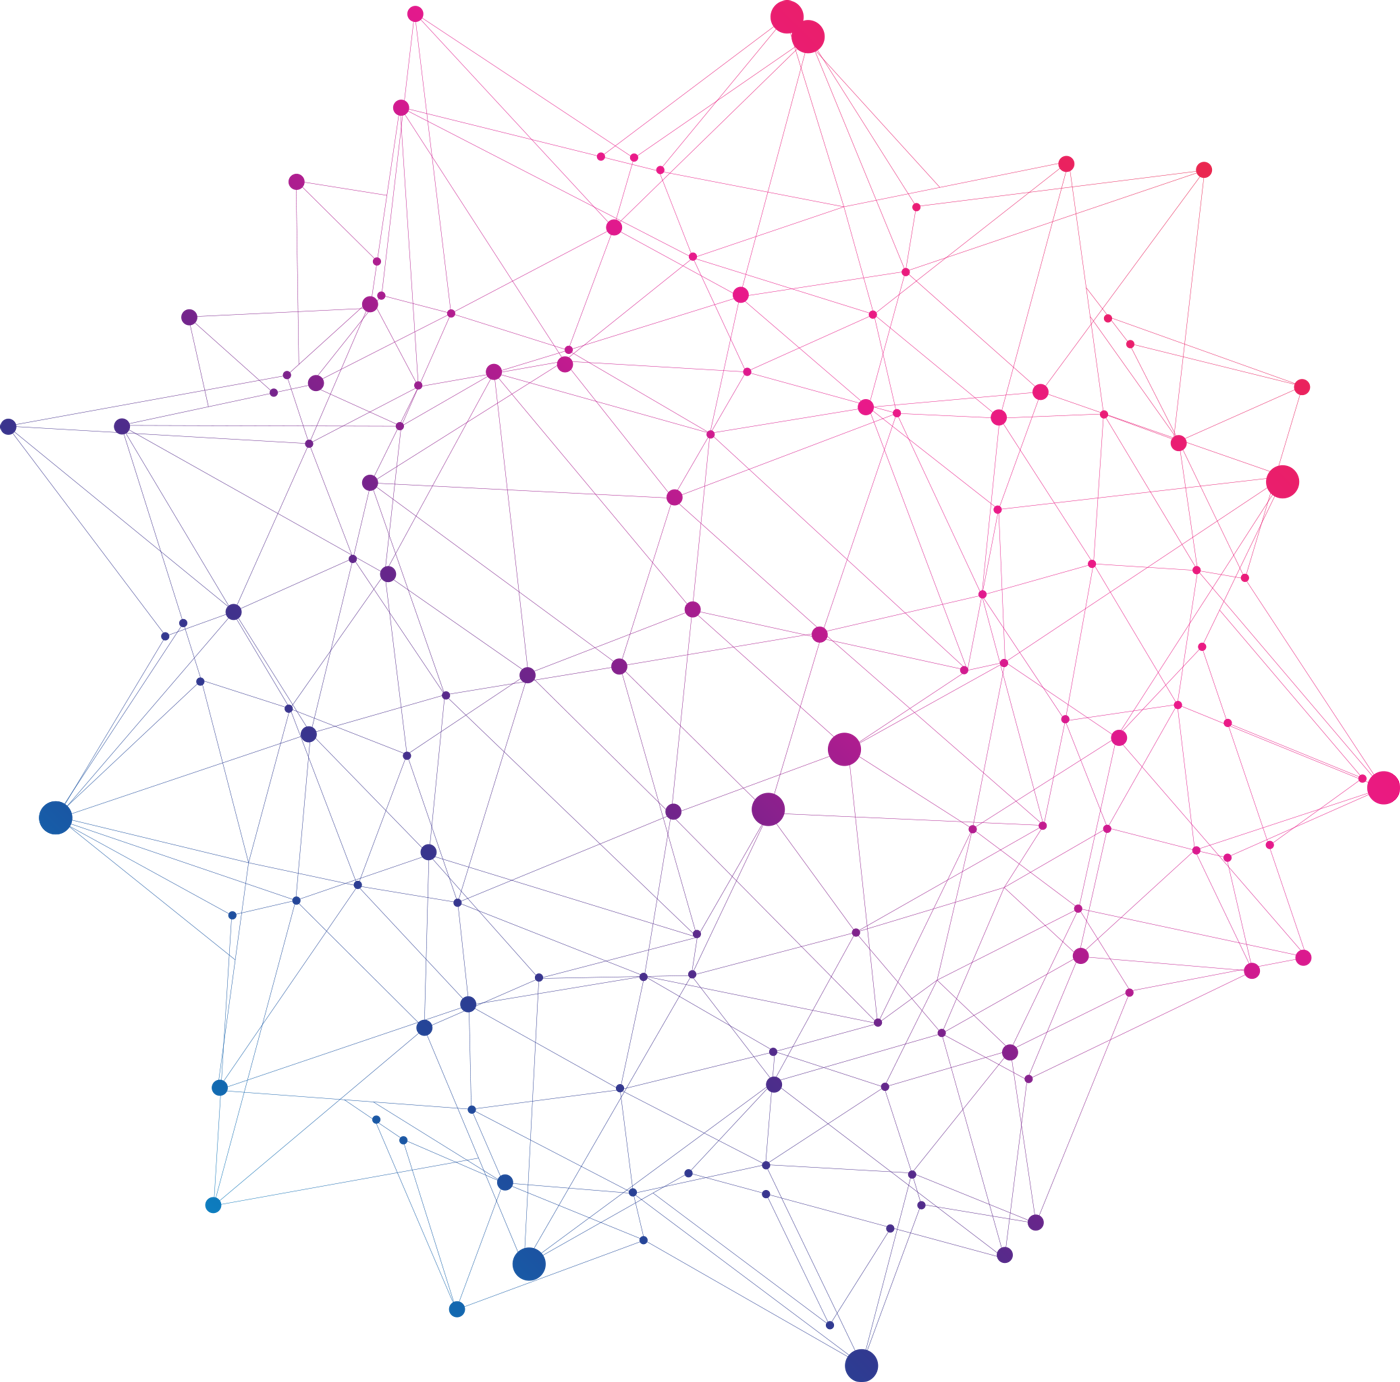
\includegraphics[width=.75\linewidth]{figures/social.png}
    \caption{The \textbf{social} environment structure.\medbreak \textit{Ex: Network}}
\end{figure}
\end{column}}
\visible<2->{\begin{column}{.33\linewidth}
\vspace{1cm}
\begin{figure}
    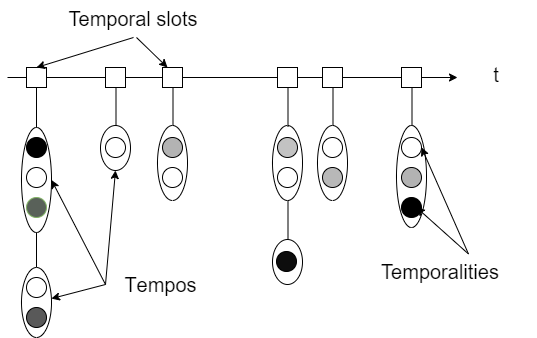
\includegraphics[width=\linewidth]{figures/temporalityModel.png}
    \caption{The \textbf{temporal} environment structure.\medbreak \textit{\alert{The temporality model}}}
\end{figure}
\vspace{.5cm}
\end{column}}
\end{columns}

\note{
Chaque environnement possède une structure et des mécaniques qui lui sont propre. Par exemple, l'environnement spatial peut être structuré à partir de données SIG, de grilles, d'espace continu, l'environnement social peut être structuré à partir de réseaux. Dans notre proposition, l'environnement temporel est structuré sur la base d'une approche appelée modèle à Temporalité.
\par Le modèle à temporalité est une approche qui à l'origine a été conçu pour l'ordonnancement de la simulation, au même titre que l'approche à pas de temps constant ou l'approche événementielle. Il permet aux agents d'exprimer leur dynamique d'activation temporelle et de les partager à l'ordonnanceur de la simulation. Au niveau de l'ordonnanceur, cette dynamique est représentée sous la forme de temporalité, agrégé à travers des tempos. Ces tempos sont rattachées à des slots temporels qui ponctuent l'axe temporel de la simulation. Une explication détaillée peut peut être lues dans nos contributions
}
    
\end{frame}

\begin{frame}{The Temporal Environment}{The Temporality Model}
\begin{figure}
    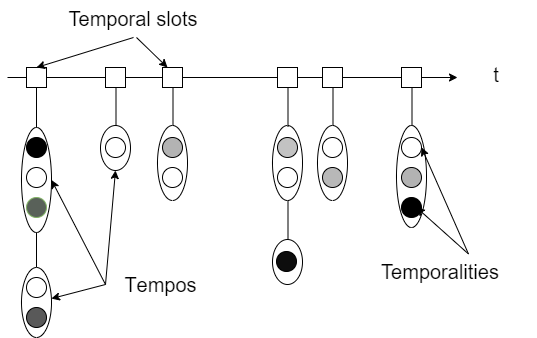
\includegraphics[width=.4\linewidth]{figures/temporalityModel.png}
    \caption{The temporality model\footnote{
PAYET, Denis, COURDIER, Rémy, RALAMBONDRAINY, Tiana, et al. Le modèle à Temporalité: pour un équilibre entre adéquation et optimisation du temps dans les simulations agent. In : JFSMA. 2006. p. 63-76.
\medbreak
RALITERA, Tahina, PAYET, Denis, AKY, Nathan, et al. The Temporality Model Time Scheduling Approach: A Practical Application. In : International Workshop on Multi-Agent Systems and Agent-Based Simulation. Springer, Cham, 2018. p. 115-125.} time axis.}
\end{figure}
\par \textbf{Model evolution} for the use in the context of the temporal environment: \alert{storage and perception} of information about the past and the future
\note{
\par Nous reprenons alors ces bases afin de structurer l'environnement temporel. Cependant, nous procédons à une extension du modèle de manière à permettre le stockage et la perception des informations sur le passé et sur le futur qui n'existait pas dans l'approche original du modèle à temporalité car cela n'était pas nécessaire compte tenu de l'objectif pour lequel il a été conçu. 
\par En effet, comme il s'agit d'une approche d'ordonnancement, l'axe temporel est située au niveau de l'ordonnanceur qui est le seul à l'exploiter. Par conséquent, seul les informations nécessaires à l'activation des agents y sont représentés et stockés. C'est à dire que les informations passées sont automatiquement effacés car elles ne servent plus à l'activation de la simulation et les informations futures sont calculées à chaque avancement du temps. Ce fonctionnement permet l'optimisation du mécanisme d'ordonnancement de la simulation.
\par Cependant, le stockage et la perception des comportements temporels passés et futurs sont indispensable dans l'usage que nous en faisons. Nous effectuons alors une refonte du modèle afin d'y intégrer ces fonctionnalités.
}
    
\end{frame}

\begin{frame}{The Temporal Environment}{Temporal information storage and perception}
\begin{figure}
    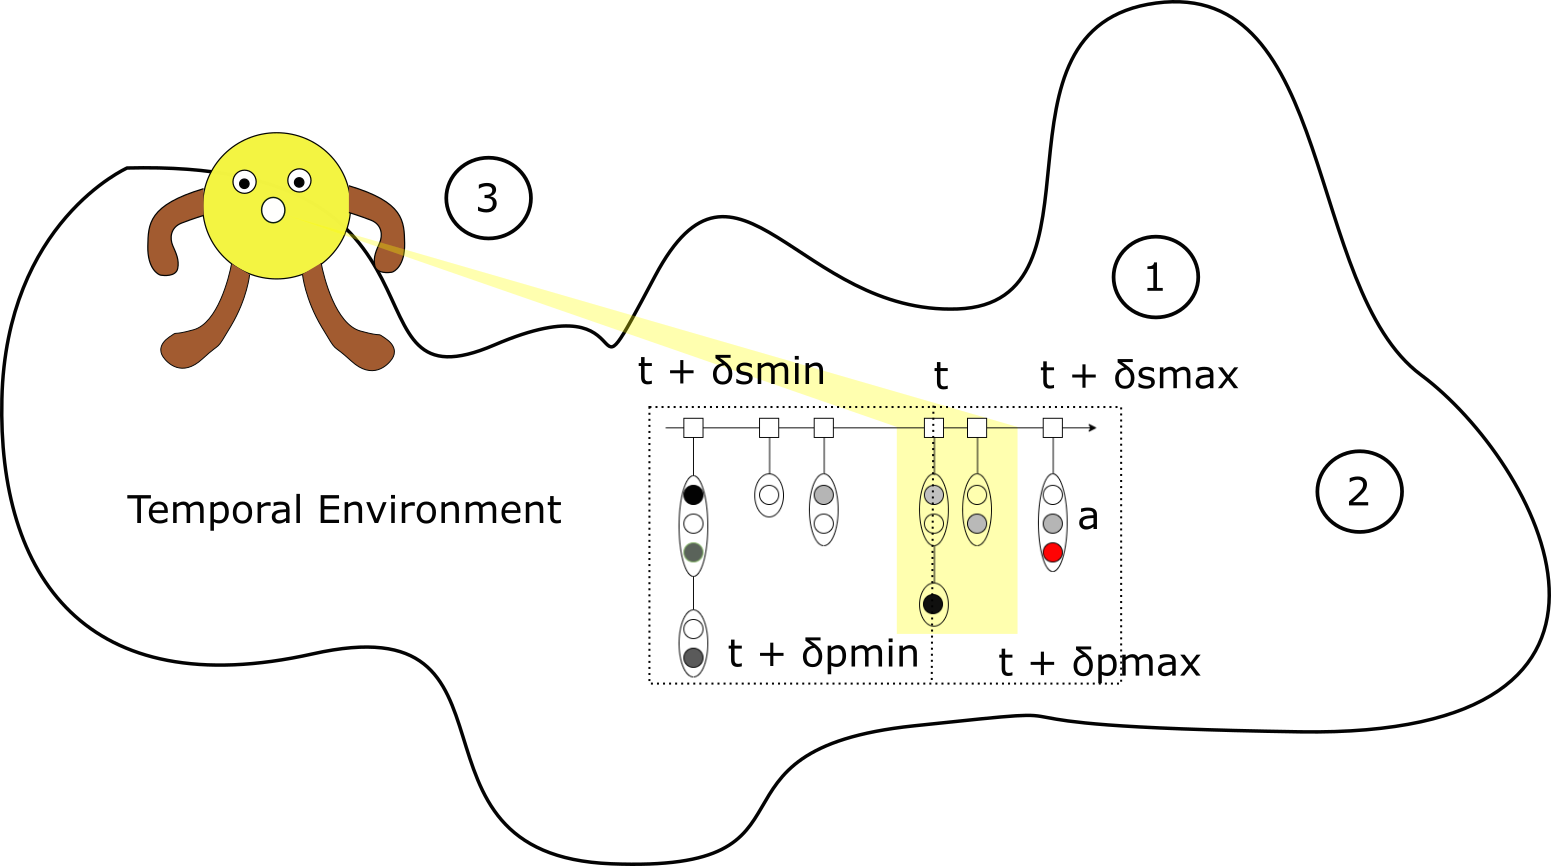
\includegraphics[width=.55\linewidth]{figures/horizon.png}
    \caption{The temporal environment: Storage and perception}
\end{figure}
\begin{enumerate}
     \item Absolute time horizon or storage time horizon of the temporal environment $[t-\delta smin,t+\delta smax]$
     \item Accessibility rules $a$. \textit{Ex: public or private}
    \item Relative time horizon or time horizon of perception of the agents $[t-\delta pmin,t+\delta pmax]$
\end{enumerate}

\note{
Afin de gérer le stockage et la perception des informations temporelles, nous mettons en oeuvre deux contraintes:
\begin{itemize}
    \item L'horizon temporel absolu ou horizon temporel de stockage de l'environnement : elle définie une portée de stockage des informations temporelles qui est commune à tous les agents de la simulation. En effet, la pertinence de ces informations varie en fonction du temps, du modèle et du type d'information. Une information passée peut avoir une durée de vie au-delà de laquelle elle devient obsolète. De même, au-delà d'une certaine limite dans le temps, une information future n'est pas forcément pertinente. L'horizon temporel absolue permet d'optimiser le stockage en ne gardant uniquement que les informations pertinentes. La valeur de ses bornes sont définies arbitrairement par l'utilisateur ou le concepteur du modèle. Dans le modèle à temporalité, au niveau de l'ordonnanceur, la valeur de l'horizon temporel absolue est nulle. Ce qui équivaut au faut que l'axe temporel ne stocke que les informations présentes. Contrairement à cela, dans l'environnement temporel, la valeur de l'horizon temporel absolu est non nulle.
    \item L'horizon temporel relative ou horizon temporel de perception des agents : elle est propre aux caractéristiques de chaque agent et contraint sa perception. Son équivalent spatiale est le champ de vision.
\end{itemize}
}
    
\end{frame}


\begin{frame}{The Temporal Environment}{Example and implementation}
\begin{figure}
    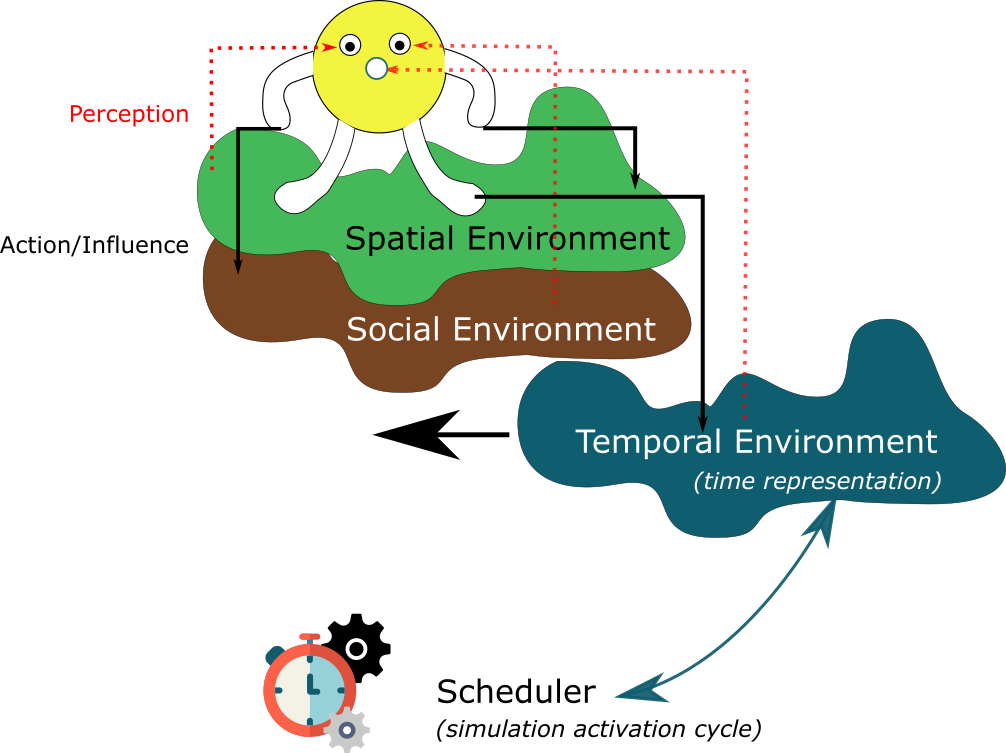
\includegraphics[width=.6\linewidth]{figures/after.png}
    \caption{Implementation of the temporal environment}
\end{figure}
\note{

\par Un autre changement, que j'ai déjà mentionné précédemment se situe au niveau du lien direct qui existait auparavant entre les agent et l'ordonnanceur de la simulation. Chaque agent communiquait directement son planning d'activité à l'ordonnanceur de la simulation qui utilisait ces informations pour activer chaque agent au moment souhaité. L'environnement temporel vient s'interfacer entre l'agent et l'ordonnanceur cassant le lien direct qui existait avant entre eux. Avant l'agent exprimait sa dynamique d'activation temporelle. Celle-ci était directement traitée au niveau de l'ordonnanceur de la simulation. Ce dernier était donc le seul à avoir accès à ces informations et l'utilisait uniquement pour la gestion de l'activation des agents et plus généralement pour la gestion du cycle d'activation de la simulation. Désormais, l'agent exprime sa dynamique d'activation temporelle, cette dernière est stockée au niveau de l'environnement temporel qui permet son accès non seulement par l'ordonnanceur de la simulation comme ce qui était déjà le cas avant mais également par les agents en fonction des horizons temporelles (absolue et relative) et d'autres règles d'accessibilité qui peuvent être définies par le modélisateur.
\par Désormais, les agents partagent leur planning au niveau de l'environnement temporel. Ce planning devient alors accessible non seulement par l'ordonnanceur mais également par les autres agents du système. Maintenant que les agents ont accès à cette information partagée sur le comportement temporel des autres agents, ils peuvent l'exploiter dans le cadre de son raisonnement. Ce qui constitue notre deuxième contribution qui consiste en l'exploitation de ces informations afin d'enrichir ceux utilisées au niveau du raisonnement anticipatif de l'agent.}

\end{frame}


\begin{frame}{The Temporal Environment}{Example and implementation \footnote{Simulation model using influence/reaction interaction model}}
\begin{columns}
\visible<1->{
\begin{column}{.4\linewidth}
\vspace{.3cm}
\begin{figure}
    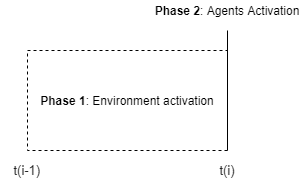
\includegraphics[width=\linewidth]{figures/old_cycle.png}
    \caption{Classical simulation activation cycle}
\end{figure}
\end{column}}
\visible<2->{
\begin{column}{.6\linewidth}
\begin{figure}
    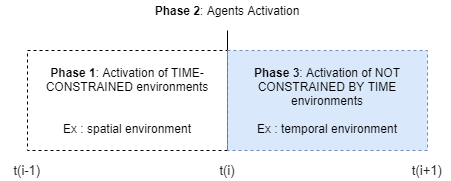
\includegraphics[width=\linewidth]{figures/new_cycle.png}
    \caption{New simulation activation cycle}
\end{figure}
\end{column}}
\end{columns}
\note{
\scriptsize{
\par La mise en place de l'environnement temporel au sein du système existant apporte de nouveaux changement. Un changement qui nous semble intéressant concerne le cycle d'activation de la simulation utilisant une approche d'interaction de type influence/réaction. Si le cycle d'activation classique consiste en 2 phases : 
\begin{itemize}
   \item Une phase d’activation de l’environnement durant laquelle le simulateur doit mettre à jour l’horloge virtuelle, initialiser le prochain cycle, etc.;
    \item Une phase d'activation des agents durant laquelle l'agent applique le processus itératif : perception, mémorisation, décision. 
\end{itemize}
L'introduction de l'environnement temporel vient chambouler ce cycle d'activation classique en scindant l'activation des environnements en deux:
\begin{itemize}
    \item L'activation des environnements contraints par le temps
    \item L'activation des environnements non contraints par le temps.
\end{itemize}
Dans la plupart des simulateurs, la phase d'activation de l'environnement se déroule en début du cycle d'activité de la simulation. Cela est dû au fait que la plupart des environnements a besoin de calculer son nouvel état en début d'un cycle (instant $t$), avant l'activation des agents. Ces calculs doivent  s'établir sur l'intervalle de temps qui s'est écoulé depuis la dernière activation. Ces environnements ont des états qui évoluent dans le temps en fonction des lois inertielles qui leur sont propres, et des influences qu'exercent les agents. Ce sont donc, en quelque sorte, des environnements contraints par le temps. Des exemple sont les environnements spatiales.
\par Dans notre contexte, par définition, l'état de l'environnement temporel détermine la dynamique d'écoulement du temps. Par conséquent, son état évolue hors du temps. \textbf{L'environnement temporel n'est donc pas un environnement contraint par le temps}. 
\par Ainsi, les 3 nouvelles phases du cycle d'activation de la simulation utilisant une approche de type influence/réaction:
\begin{enumerate}
    \item la phase d'activation des environnements contraints par le temps sur l'intervalle de temps $] ]t(i-1), t(i)]$; 
    \item la phase d'activation des agents sur le slot temporel courant $t$;
    \item la phase d'activation des environnements non contraints par le temps sur la considération que $t$ vient d'être passé.
\end{enumerate}
}
}
\end{frame}


